\documentclass[tikz,border=4pt]{standalone}
\usepackage{pgfplots}\usepgfplotslibrary{groupplots}
\pgfplotsset{compat=1.18}
\definecolor{corba}{HTML}{365FB3}\definecolor{guia}{HTML}{7C3AED}\definecolor{punt}{HTML}{B91C1C}
\begin{document}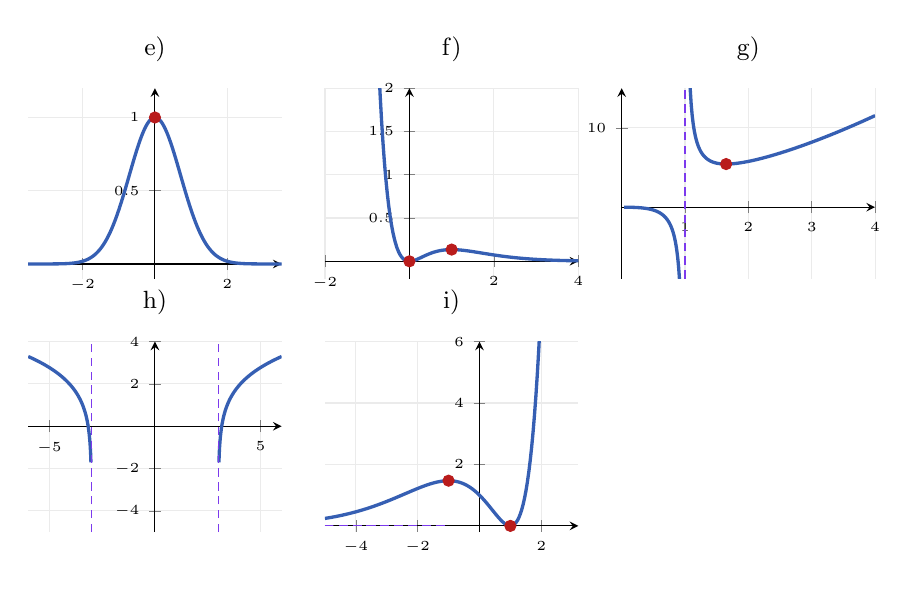
\begin{tikzpicture}
\begin{groupplot}[group style={group size=3 by 2,horizontal sep=0.55cm,vertical sep=0.8cm},width=4.8cm,height=4cm,
 axis lines=middle,grid=major,grid style={black!8},tick label style={font=\tiny},title style={font=\small},samples=180]
\nextgroupplot[title={e)},xmin=-3.5,xmax=3.5,ymin=-.1,ymax=1.2]\addplot[corba,very thick,domain=-3.5:3.5]{exp(-x^2)};\addplot[only marks,mark=*,punt] coordinates {(0,1)};
\nextgroupplot[title={f)},xmin=-2,xmax=4,ymin=-.2,ymax=2]\addplot[corba,very thick,domain=-2:4]{x^2*exp(-2*x)};\addplot[only marks,mark=*,punt] coordinates {(0,0)(1,.1353)};
\nextgroupplot[title={g)},xmin=0,xmax=4,ymin=-9,ymax=15]\addplot[corba,very thick,domain=.04:.97]{x^2/ln(x)};\addplot[corba,very thick,domain=1.03:4]{x^2/ln(x)};\addplot[guia,densely dashed] coordinates {(1,-9)(1,15)};\addplot[only marks,mark=*,punt] coordinates {(1.6487,5.4366)};
\nextgroupplot[title={h)},xmin=-6,xmax=6,ymin=-5,ymax=4]\addplot[corba,very thick,domain=-6:-3.03]{ln(x^2-9)};\addplot[corba,very thick,domain=3.03:6]{ln(x^2-9)};\addplot[guia,densely dashed] coordinates {(-3,-5)(-3,4)};\addplot[guia,densely dashed] coordinates {(3,-5)(3,4)};
\nextgroupplot[title={i)},xmin=-5,xmax=3.2,ymin=-.2,ymax=6]\addplot[corba,very thick,domain=-5:3.2]{(x-1)^2*exp(x)};\addplot[guia,densely dashed,domain=-5:-1]{0};\addplot[only marks,mark=*,punt] coordinates {(-1,1.4715)(1,0)};
\end{groupplot}\end{tikzpicture}\end{document}
